%First stage



\begin{figure}[htbp]
    \centering
    
    \begin{subfigure}{\textwidth}
        \centering
        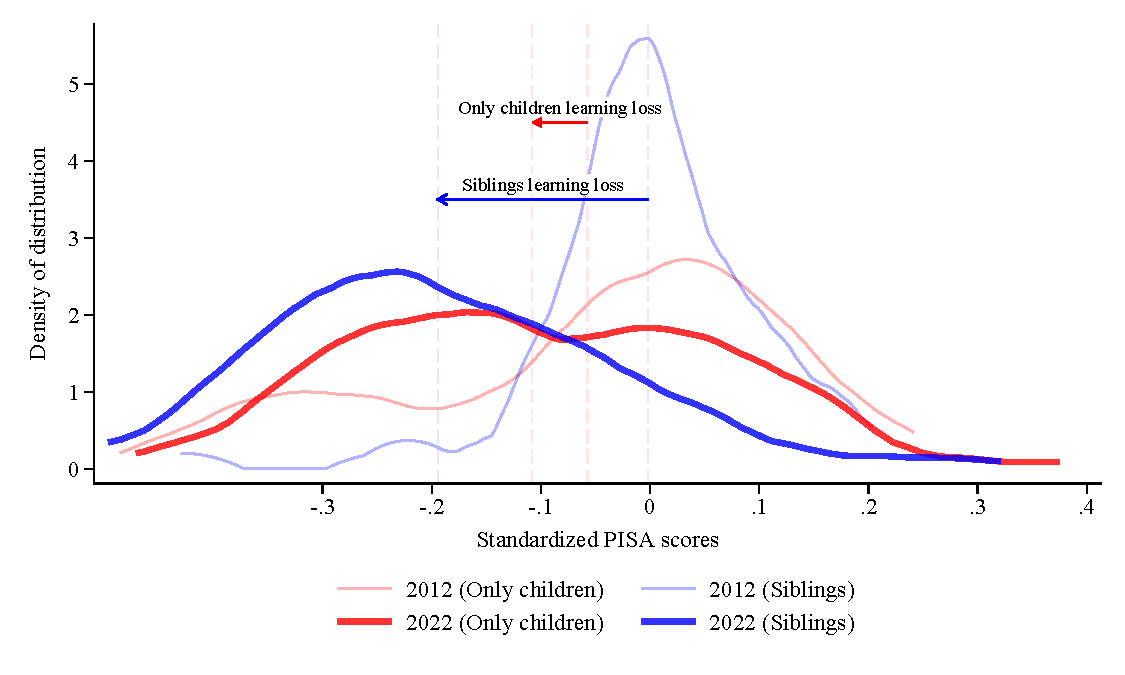
\includegraphics[width=\textwidth]{./FIGURES/Descriptive/PISA_distribution_2012_2022_PV4MATH.pdf}
        \caption{Learning gaps in Mathematics between 2012 and 2022 for only children and children with siblings}
        \label{fig:1a}
    \end{subfigure}
    
    \vspace{1em} % Add some vertical space between subfigures
    
    \begin{subfigure}{\textwidth}
        \centering
        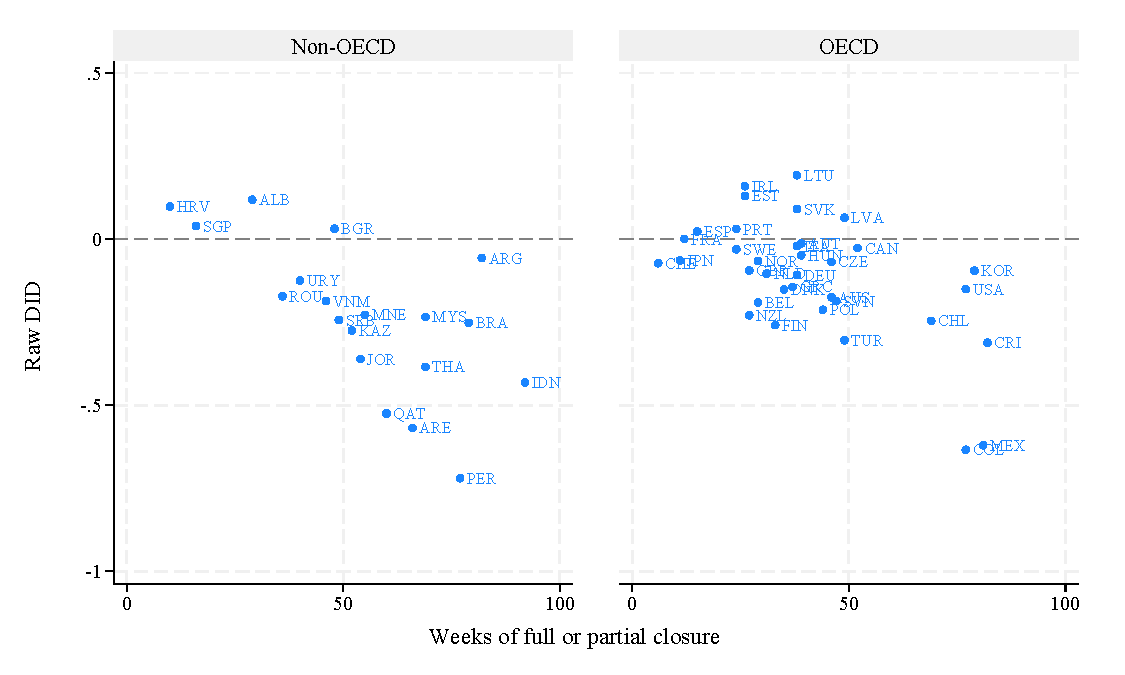
\includegraphics[width=\textwidth]{./FIGURES/Descriptive/PISA_raw_DID_PV4MATH_not_fully_open.pdf}
        \caption{Change in learning gaps by duration of school closure for OECD and Non-OECD countries.}
        \label{fig:1b}
    \end{subfigure}
    
    \caption{Learning gaps around the world}
    \label{fig:pisa}
\end{figure}



\begin{figure}[htbp]
    \centering
    
    \begin{subfigure}{\textwidth}
        \centering
        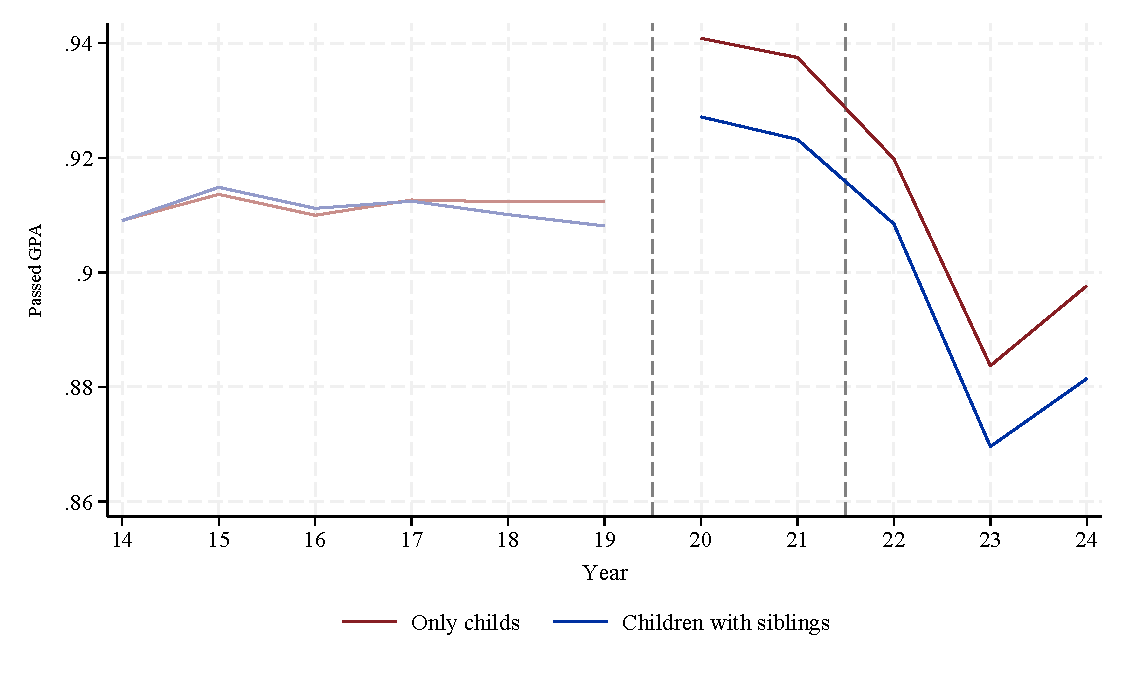
\includegraphics[width=\textwidth]{./FIGURES/Descriptive/raw_total_elm_pass_math_siblings.pdf}
        \caption{\% of students with a A in Mathematics from 1st-6th grade}
        \label{fig:trend_pass}
    \end{subfigure}
    
    \vspace{1em} % Add some vertical space between subfigures
    
    \begin{subfigure}{\textwidth}
        \centering
        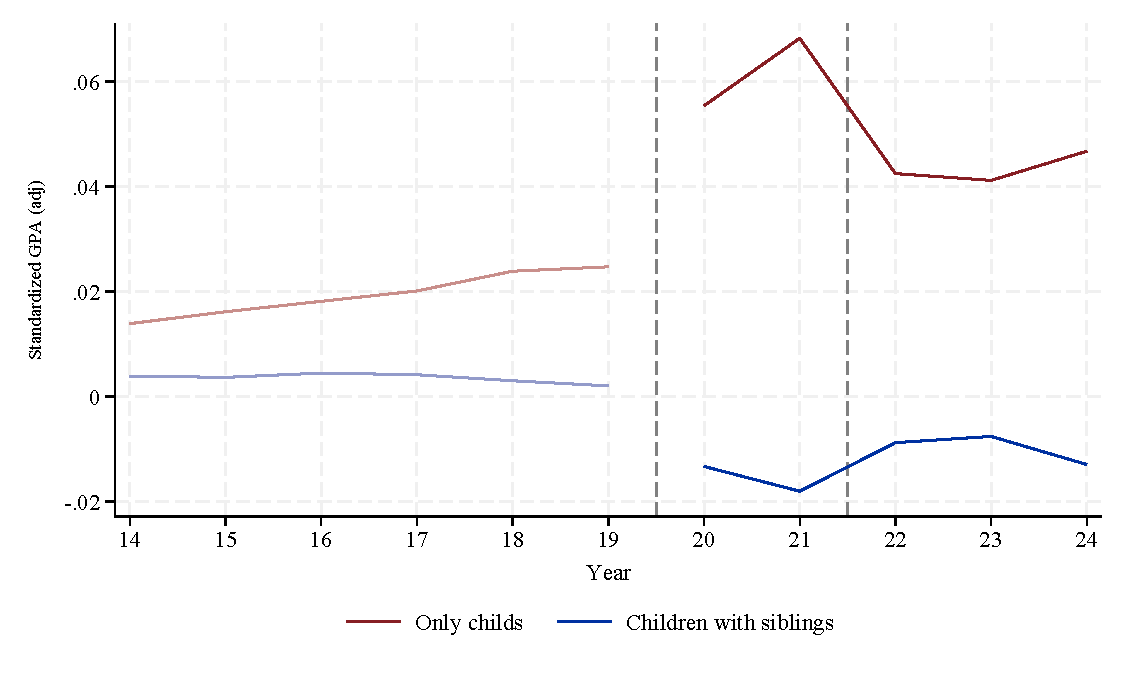
\includegraphics[width=\textwidth]{./FIGURES/Descriptive/raw_total_elm_std_gpa_m_adj_siblings.pdf}
        \caption{Average GPA standardized within school-grade-year from 1st-6th grade}
        \label{fig:trend_gpa}
    \end{subfigure}
    
    \caption{Trends in education outcomes for only children and children with siblings}
    \label{fig:trend}
\end{figure}


\begin{figure}[htbp]
    \centering
    
    \begin{subfigure}{\textwidth}
        \centering
        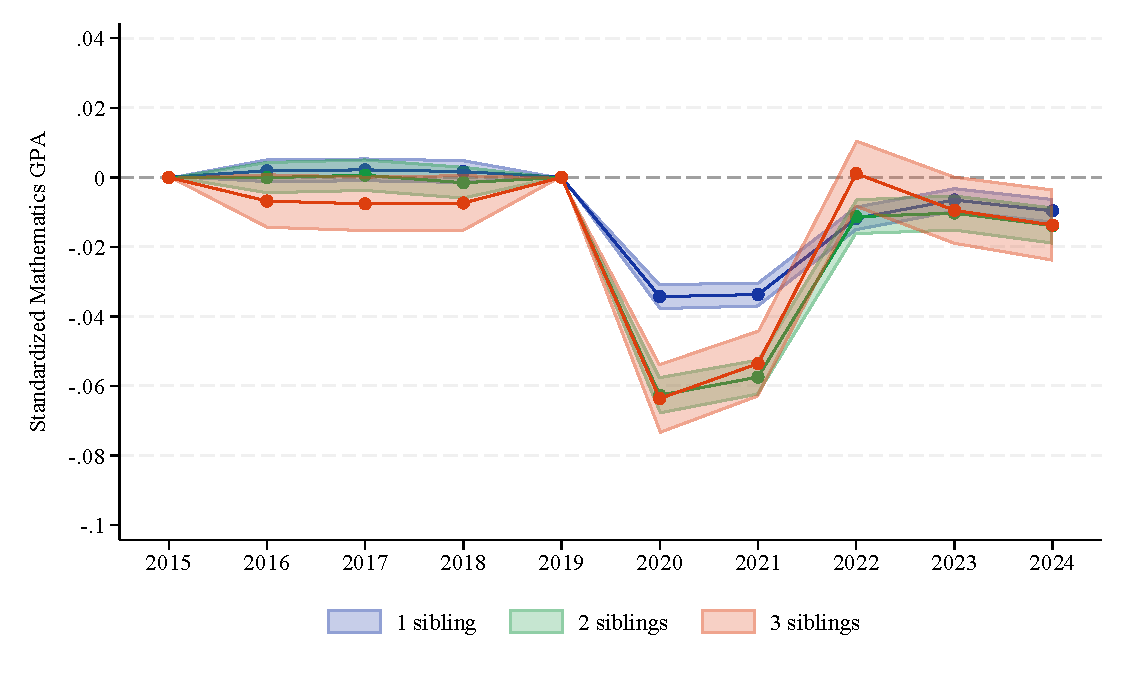
\includegraphics[width=\textwidth]{./FIGURES/Event Study/covid_event_bysibs_all_all_std_gpa_m_adj_Tsiblings_Soldest_4.pdf}
        \caption{Event Study - Learning losses compared to only children by number of siblings}
        \label{fig:main_result_event}
    \end{subfigure}
    
    \vspace{1em} % Add some vertical space between subfigures
    
    \begin{subfigure}{\textwidth}
        \centering
        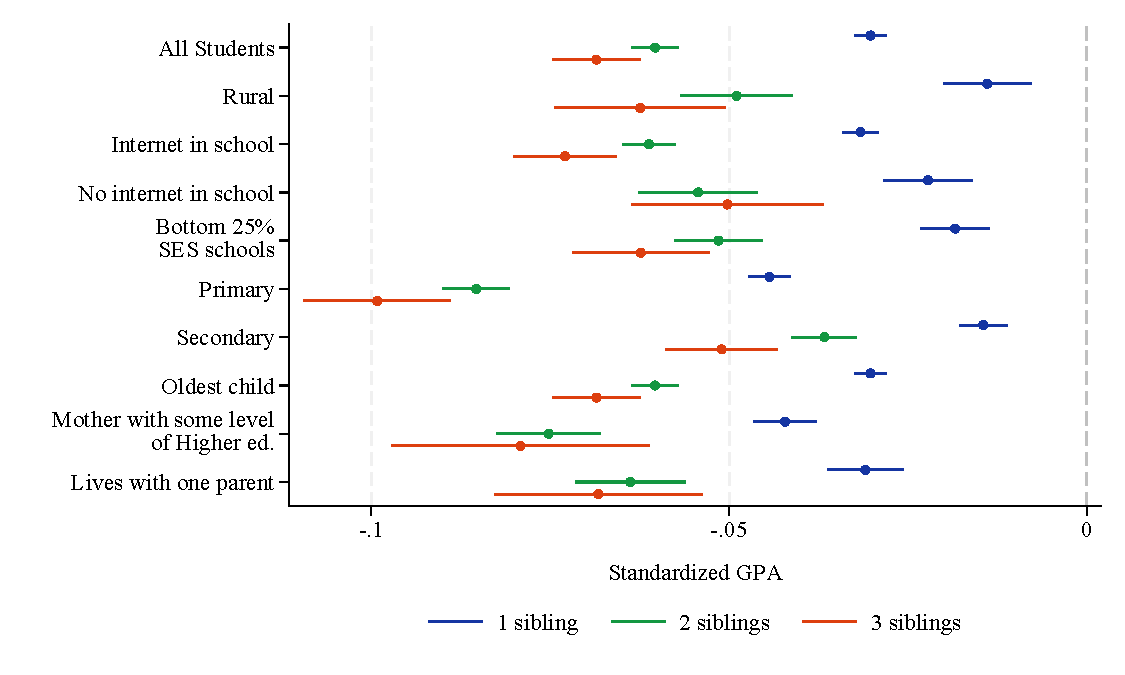
\includegraphics[width=\textwidth]{./FIGURES/TWFE/covid_twfe_summ_bysibs_all_20-21_gpa_m_adj_Tsiblings_Soldest_4.pdf}
        \caption{Change in gap between children with siblings and only childs}
        \label{fig:main_result_twfe}
    \end{subfigure}
    
    \caption{Learning gap between only childs and siblings}
    \label{fig:main_result}
\end{figure}


\clearpage

%RD-first grade
\makeatletter
\@ifclassloaded{beamer}{%
       \centering
       \resizebox{0.5\textwidth}{!}%
}{%
       \begin{table}[!tbp]\centering\def\sym#1{\ifmmode^{#1}\else\(^{#1}\)\fi}
       \centering
       \caption{Descriptive Statistics}
       \label{tab:descriptive}
       \resizebox{0.8\textwidth}{!}%
}
{
\makeatother
\begin{tabular}{lcccc}
\toprule
& Only children & 1 sibling & 2 siblings & 3 siblings  \\
\cmidrule(lr){2-2} \cmidrule(lr){3-3} \cmidrule(lr){4-4} \cmidrule(lr){5-5}
& (1) & (2) & (3) & (4)\\
\bottomrule
&  &  &  & \\
            &            &            &            &            \\
\% of sample &       0.570&       0.271&       0.122&       0.037\\
&  &  &   \\
\multicolumn{4}{l}{\textit{Panel A: School and student characteristics}} \\
            &            &            &            &            \\
\% Urban    &       0.773&       0.800&       0.741&       0.621\\
\% Public School&       0.657&       0.660&       0.749&       0.852\\
%Average Grade&       2.000&       2.000&       2.000&       2.000\\
\% Male     &       0.513&       0.514&       0.511&       0.514\\
&  &  &   \\
\multicolumn{4}{l}{\textit{Panel B: Academic characteristics}} \\
            &            &            &            &            \\
\% Grade promotion&       0.931&       0.952&       0.934&       0.897\\
\% Grade promotion without recovery&       0.878&       0.903&       0.884&       0.848\\
Standardized GPA (Mathematics) &       0.025&       0.097&       0.030&      -0.061\\
Standardized GPA (Reading)&       0.030&       0.099&       0.032&      -0.060\\
&  &  &   \\
\multicolumn{4}{l}{\textit{Panel C: Parent's characteristics}} \\
            &            &            &            &            \\
\% Lives with both parents&       0.583&       0.649&       0.618&       0.575\\
\% Lives with one parent&       0.197&       0.184&       0.189&       0.193\\
\% Lives with Mother&       0.807&       0.821&       0.798&       0.764\\
\% Lives with Father&       0.698&       0.740&       0.719&       0.687\\
\% Father without complete secondary&       0.324&       0.278&       0.348&       0.480\\
\% Father with complete secondary&       0.416&       0.438&       0.436&       0.391\\
\% Father with some level of higher ed.&       0.259&       0.284&       0.215&       0.129\\
\% Mother without complete secondary&       0.368&       0.331&       0.413&       0.563\\
\% Mother with complete secondary&       0.395&       0.418&       0.408&       0.346\\
\% Mother with some level of higher ed.&       0.237&       0.251&       0.178&       0.090\\
&  &  &   \\
\multicolumn{4}{l}{\textit{Panel D: Household Resources (2nd grade: 2015, 2016)}} \\
            &            &            &            &            \\
SES         &       0.102&       0.065&      -0.130&      -0.394\\
%HH size     &       5.007&       5.058&       5.399&       5.847\\
%\# of bedrooms&       2.853&       2.673&       2.613&       2.672\\
\% Radio    &       0.831&       0.822&       0.789&       0.758\\
\% Internet &       0.334&       0.300&       0.234&       0.149\\
\% PC       &       0.345&       0.317&       0.243&       0.160\\
\% Laptop   &       0.308&       0.284&       0.219&       0.141\\
\% 6+ books &       0.567&       0.521&       0.450&       0.370\\
\% Quiet room to study&       0.859&       0.854&       0.827&       0.794\\
&  &  &   \\
\multicolumn{4}{l}{\textit{Panel E: Academic Performance (2nd grade: 2015, 2016)}} \\
            &            &            &            &            \\
standardized Reading score&       0.930&       0.997&       0.872&       0.661\\
standardized Mathematics score&       0.883&       0.995&       0.883&       0.676\\
Did 3 years of Pre-K&       0.656&       0.665&       0.640&       0.566\\
Has repeated a grade&       0.043&       0.033&       0.044&       0.071\\
&  &  &   \\
\multicolumn{4}{l}{\textit{Panel F: Parent's Characteristics (2nd grade: 2015, 2016)}} \\
            &            &            &            &            \\
\% Mother with complete secondary&       0.245&       0.273&       0.276&       0.261\\
\% Mother with some level of higher ed&       0.375&       0.397&       0.309&       0.192\\
\% Spanish  &       0.866&       0.862&       0.847&       0.829\\
\%Education expectation: High School&       0.096&       0.080&       0.105&       0.163\\
\%Education expectation: 4-year college&       0.791&       0.817&       0.765&       0.668\\

\bottomrule
\end{tabular}
}
\@ifclassloaded{beamer}{%
}{%
       \end{table}
}

%\makeatletter
\@ifclassloaded{beamer}{%
       \centering
       \resizebox{0.5\textwidth}{!}%
}{%
       \begin{table}[!tbp]\centering\def\sym#1{\ifmmode^{#1}\else\(^{#1}\)\fi}
       \centering
       \caption{Descriptive Statistics}
       \label{tab:descriptive}
       \resizebox{0.8\textwidth}{!}%
}
{
\makeatother
\begin{tabular}{lcccc}
\toprule
\cmidrule(lr){2-4}
& \multicolumn{4}{c}{TWFE}  \\
\cmidrule(lr){2-4}
& Only children & 1 sibling & 2 siblings & 3 siblings  \\
\cmidrule(lr){2-2} \cmidrule(lr){3-3} \cmidrule(lr){4-4} \cmidrule(lr){5-5}
& (1) & (2) & (3) & (4)\\
\bottomrule
&  &  &  & \\
&  &  &   \\
\multicolumn{4}{l}{\textit{Panel A: School and student characteristics}} \\
            &            &            &            &            \\
\% Urban    &       0.812&       0.814&       0.752&       0.645\\
\% Public School&       0.681&       0.702&       0.793&       0.879\\
Average Grade&       6.072&       5.952&       6.460&       6.910\\
\% Male     &       0.511&       0.512&       0.510&       0.506\\
&  &  &   \\
\multicolumn{4}{l}{\textit{Panel B: Academic characteristics}} \\
            &            &            &            &            \\
\% Grade promotion&       0.953&       0.963&       0.947&       0.920\\
\% Grade promotion without recovery&       0.826&       0.842&       0.799&       0.753\\
Standardized GPA (Mathematics) &       0.016&       0.072&       0.006&      -0.073\\
Standardized GPA (Reading)&       0.022&       0.071&      -0.001&      -0.083\\
&  &  &   \\
\multicolumn{4}{l}{\textit{Panel C: Parent's characteristics}} \\
            &            &            &            &            \\
\% Lives with both parents&       0.493&       0.558&       0.555&       0.536\\
\% Lives with one parent&       0.178&       0.170&       0.178&       0.179\\
\% Lives with Mother&       0.768&       0.768&       0.766&       0.747\\
\% Lives with Father&       0.670&       0.700&       0.694&       0.682\\
\% Father without complete secondary&       0.302&       0.272&       0.355&       0.490\\
\% Father with complete secondary&       0.428&       0.443&       0.428&       0.377\\
\% Father with some level of higher ed.&       0.270&       0.286&       0.217&       0.133\\
\% Father without complete secondary&       0.343&       0.323&       0.421&       0.569\\
\% Father with complete secondary&       0.413&       0.425&       0.401&       0.334\\
\% Father with some level of higher ed.&       0.244&       0.252&       0.179&       0.097\\
&  &  &   \\
\multicolumn{4}{l}{\textit{Panel D: Household Resources (2nd grade: 2015, 2016)}} \\
            &            &            &            &            \\
SES         &       0.122&       0.079&      -0.114&      -0.378\\
HH size     &       4.949&       5.035&       5.435&       5.876\\
\# of bedrooms&       2.846&       2.664&       2.604&       2.661\\
\% Radio    &       0.683&       0.653&       0.690&       0.704\\
\% Internet &       0.416&       0.415&       0.345&       0.243\\
\% PC       &       0.454&       0.458&       0.365&       0.258\\
\% Laptop   &       0.405&       0.412&       0.338&       0.242\\
\% 6+ books &       0.574&       0.527&       0.457&       0.377\\
\% Quiet room to study&       0.861&       0.855&       0.829&       0.796\\
&  &  &   \\
\multicolumn{4}{l}{\textit{Panel E: Academic Performance (2nd grade: 2015, 2016)}} \\
            &            &            &            &            \\
standardized Reading score&       0.702&       0.756&       0.621&       0.397\\
standardized Mathematics score&       0.608&       0.691&       0.570&       0.361\\
Did 3 years of Pre-K&       0.660&       0.668&       0.645&       0.572\\
Has repeated a grade&       0.035&       0.027&       0.037&       0.058\\
&  &  &   \\
\multicolumn{4}{l}{\textit{Panel F: Parent's Characteristics (2nd grade: 2015, 2016)}} \\
            &            &            &            &            \\
\% Mother with complete secondary&       0.251&       0.278&       0.279&       0.266\\
\% Mother with 4-year college&       0.398&       0.415&       0.318&       0.193\\
\% Spanish  &       0.866&       0.861&       0.847&       0.828\\
\%Education expectation: High School&       0.084&       0.071&       0.100&       0.159\\
\%Education expectation: 4-year college&       0.808&       0.828&       0.769&       0.671\\

\bottomrule
\end{tabular}
}
\@ifclassloaded{beamer}{%
}{%
       \end{table}
}



\makeatletter
\@ifclassloaded{beamer}{%
       \centering
       \resizebox{0.6\textwidth}{!}%
}{%
       \begin{table}[!tbp]\centering\def\sym#1{\ifmmode^{#1}\else\(^{#1}\)\fi}
       \centering
       \caption{TWFE on 8th grade GPA and standardized exams controlling for baseline 2nd grade standardized exams}
       \label{tab:twfe_ece}
       \resizebox{0.95\textwidth}{!}%
}
{
\makeatother
\begin{tabular}{lcccc}
\toprule
\cmidrule(lr){2-5}
& \multicolumn{4}{c}{TWFE} \\
\cmidrule(lr){2-5}
& 1-3 siblings & 1 sibling & 2 siblings & 3 siblings  \\
\cmidrule(lr){2-2} \cmidrule(lr){3-3} \cmidrule(lr){4-4} \cmidrule(lr){5-5}
& (1) & (2) & (3) & (4) \\
\bottomrule
&  &  & &  \\
&  &  & &  \\
\multicolumn{5}{l}{Panel A: GPA } \\
Mathematics         &      -0.099***&      -0.011   &      -0.036***&      -0.059***\\
                    &     (0.009)   &     (0.009)   &     (0.011)   &     (0.015)   \\
                    &               &               &               &               \\
Observations        &     326,669   &     279,833   &     225,092   &     179,575   \\
 
&  &  & &  \\
Reading             &      -0.099***&      -0.010   &      -0.031***&      -0.034** \\
                    &     (0.009)   &     (0.009)   &     (0.010)   &     (0.015)   \\
                    &               &               &               &               \\
Observations        &     326,669   &     280,846   &     225,840   &     180,218   \\
 
&  &  & &  \\
\multicolumn{5}{l}{Panel B: Standardized Exams } \\
Mathematics         &      -0.034***&      -0.017** &      -0.044***&      -0.071***\\
                    &     (0.006)   &     (0.007)   &     (0.008)   &     (0.011)   \\
                    &               &               &               &               \\
Observations        &     409,527   &     282,640   &     227,403   &     181,370   \\
 
&  &  & &  \\
Reading             &      -0.013** &       0.002   &      -0.022***&      -0.046***\\
                    &     (0.006)   &     (0.006)   &     (0.008)   &     (0.011)   \\
                    &               &               &               &               \\
Observations        &     409,690   &     282,769   &     227,486   &     181,466   \\
 

\bottomrule
\end{tabular}
}
\@ifclassloaded{beamer}{%
}{%
       \end{table}
}

\makeatletter
\@ifclassloaded{beamer}{%
       \centering
       \resizebox{0.6\textwidth}{!}%
}{%
       \begin{table}[!tbp]\centering\def\sym#1{\ifmmode^{#1}\else\(^{#1}\)\fi}
       \centering
       \caption{TWFE on GPA by baseline resources}
       \label{tab:twfe_gpa_baseline_survey_1_pairall}
       \resizebox{0.65\textwidth}{!}%
}
{
\makeatother
\begin{tabular}{lccc}
\toprule
\cmidrule(lr){2-4}
& \multicolumn{3}{c}{TWFE} \\
\cmidrule(lr){2-4}
& 1 sibling & 2 siblings & 3 siblings  \\
\cmidrule(lr){2-2} \cmidrule(lr){3-3} \cmidrule(lr){4-4}
& (1) & (2) & (3)\\
\bottomrule
&  &  &  \\
&  &  &   \\
\multicolumn{4}{l}{\textit{Panel A: All studentes}} \\
\hspace{3mm}Mathematics&      -0.028***&      -0.061***&      -0.080***\\
                    &     (0.004)   &     (0.005)   &     (0.009)   \\
 
%&  &  &   \\
\hspace{3mm}Reading &      -0.018***&      -0.044***&      -0.052***\\
                    &     (0.004)   &     (0.005)   &     (0.009)   \\
                    &               &               &               \\
\hspace{3mm}Observations&   1,285,073   &   1,038,874   &     906,608   \\
 
&  &  &   \\
\multicolumn{4}{l}{\textit{Panel B: Low SES Households (Q1)}} \\
\hspace{3mm}Mathematics&      -0.009   &      -0.028***&      -0.061***\\
                    &     (0.007)   &     (0.009)   &     (0.014)   \\
 
%&  &  &   \\
\hspace{3mm}Reading &      -0.003   &      -0.016*  &      -0.040***\\
                    &     (0.007)   &     (0.009)   &     (0.014)   \\
                    &               &               &               \\
\hspace{3mm}Observations&     312,464   &     264,200   &     226,444   \\
 
&  &  &   \\
\multicolumn{4}{l}{\textit{Panel C: High SES Households (Q4)}} \\
\hspace{3mm}Mathematics&      -0.037***&      -0.065***&      -0.113***\\
                    &     (0.008)   &     (0.014)   &     (0.034)   \\
 
%&  &  &   \\
\hspace{3mm}Reading &      -0.029***&      -0.070***&      -0.017   \\
                    &     (0.008)   &     (0.014)   &     (0.034)   \\
                    &               &               &               \\
\hspace{3mm}Observations&     257,212   &     199,735   &     179,355   \\
 
&  &  &   \\
\multicolumn{4}{l}{\textit{Panel D: Households with no PC or Internet}} \\
\hspace{3mm}Mathematics&      -0.032***&      -0.079***&      -0.067***\\
                    &     (0.006)   &     (0.009)   &     (0.019)   \\
 
%&  &  &   \\
\hspace{3mm}Reading &      -0.023***&      -0.056***&      -0.051***\\
                    &     (0.006)   &     (0.009)   &     (0.019)   \\
                    &               &               &               \\
\hspace{3mm}Observations&     454,966   &     366,342   &     320,367   \\
 
&  &  &   \\
\multicolumn{4}{l}{\textit{Panel E: Households with both PC and Internet}} \\
\hspace{3mm}Mathematics&      -0.023***&      -0.035***&      -0.098***\\
                    &     (0.006)   &     (0.009)   &     (0.015)   \\
 
%&  &  &   \\
\hspace{3mm}Reading &      -0.008   &      -0.039***&      -0.061***\\
                    &     (0.006)   &     (0.009)   &     (0.015)   \\
                    &               &               &               \\
\hspace{3mm}Observations&     438,221   &     355,035   &     307,508   \\
 

\bottomrule
\end{tabular}
}
\@ifclassloaded{beamer}{%
}{%
       \end{table}
}

\makeatletter
\@ifclassloaded{beamer}{%
       \centering
       \resizebox{0.6\textwidth}{!}%
}{%
       \begin{table}[!tbp]\centering\def\sym#1{\ifmmode^{#1}\else\(^{#1}\)\fi}
       \centering
       \caption{WFE on GPA by baseline achievement and expectations}
       \label{tab:twfe_gpa_baseline_survey_2_pairall}
       \resizebox{0.65\textwidth}{!}%
}
{
\makeatother
\begin{tabular}{lccc}
\toprule
\cmidrule(lr){2-4}
& \multicolumn{3}{c}{TWFE} \\
\cmidrule(lr){2-4}
& 1 sibling & 2 siblings & 3 siblings  \\
\cmidrule(lr){2-2} \cmidrule(lr){3-3} \cmidrule(lr){4-4}
& (1) & (2) & (3)\\
\bottomrule
&  &  &  \\
&  &  &   \\
\multicolumn{4}{l}{\textit{Panel A: All studentes}} \\
\hspace{3mm}Mathematics&      -0.028***&      -0.061***&      -0.080***\\
                    &     (0.004)   &     (0.005)   &     (0.009)   \\
 
%&  &  &   \\
\hspace{3mm}Reading &      -0.018***&      -0.044***&      -0.052***\\
                    &     (0.004)   &     (0.005)   &     (0.009)   \\
                    &               &               &               \\
\hspace{3mm}Observations&   1,285,073   &   1,038,874   &     906,608   \\
 
&  &  &   \\
\multicolumn{4}{l}{\textit{Panel B: Student in bottom quartile of achievement}} \\
\hspace{3mm}Mathematics&       0.001   &      -0.042***&      -0.106***\\
                    &     (0.007)   &     (0.010)   &     (0.015)   \\
 
%&  &  &   \\
\hspace{3mm}Reading &       0.009   &      -0.036***&      -0.064***\\
                    &     (0.008)   &     (0.010)   &     (0.016)   \\
                    &               &               &               \\
\hspace{3mm}Observations&     261,349   &     220,666   &     193,655   \\
 
&  &  &   \\
\multicolumn{4}{l}{\textit{Panel C: Student in top quartile of achievement}} \\
\hspace{3mm}Mathematics&      -0.045***&      -0.101***&      -0.140***\\
                    &     (0.007)   &     (0.011)   &     (0.023)   \\
 
%&  &  &   \\
\hspace{3mm}Reading &      -0.032***&      -0.069***&      -0.090***\\
                    &     (0.007)   &     (0.011)   &     (0.023)   \\
                    &               &               &               \\
\hspace{3mm}Observations&     364,927   &     282,401   &     245,220   \\
 
&  &  &   \\
\multicolumn{4}{l}{\textit{Panel D: Max Expectation: Finish school}} \\
\hspace{3mm}Mathematics&      -0.003   &      -0.030   &      -0.054*  \\
                    &     (0.014)   &     (0.019)   &     (0.030)   \\
 
%&  &  &   \\
\hspace{3mm}Reading &      -0.027*  &      -0.031   &      -0.059*  \\
                    &     (0.015)   &     (0.019)   &     (0.031)   \\
                    &               &               &               \\
\hspace{3mm}Observations&      84,652   &      71,387   &      61,974   \\
 
&  &  &   \\
\multicolumn{4}{l}{\textit{Panel E: Max Expectation: 4-year college or grad school}} \\
\hspace{3mm}Mathematics&      -0.033***&      -0.067***&      -0.095***\\
                    &     (0.004)   &     (0.006)   &     (0.011)   \\
 
%&  &  &   \\
\hspace{3mm}Reading &      -0.022***&      -0.049***&      -0.073***\\
                    &     (0.004)   &     (0.006)   &     (0.011)   \\
                    &               &               &               \\
\hspace{3mm}Observations&   1,039,027   &     830,658   &     724,846   \\
 

\bottomrule
\end{tabular}
}
\@ifclassloaded{beamer}{%
}{%
       \end{table}
}



\clearpage
\makeatletter
\@ifclassloaded{beamer}{%
       \centering
       \resizebox{0.6\textwidth}{!}%
}{%
       \begin{table}[!tbp]\centering\def\sym#1{\ifmmode^{#1}\else\(^{#1}\)\fi}
       \centering
       \caption{Effects of younger sibling delaying school on older sibling standardized exams - 1 - m - a -  - 365}
       \label{tab:rd_summ_1_m_a_365}
       \resizebox{0.95\textwidth}{!}%
}
{
\makeatother
\resizebox{\textwidth}{!}{
\begin{tabular}{lccc}
\toprule
\cmidrule(lr){2-4}
& \multicolumn{3}{c}{Standardized GPA} \\
\cmidrule(lr){2-4}
& Pre-Covid & Covid & Post-Covid  \\
& 2018-2019 & 2020-2021 & 2022-2023  \\
\cmidrule(lr){2-2} \cmidrule(lr){3-3} \cmidrule(lr){4-4}
& (1) & (2) & (3)  \\
\bottomrule
&  &  &   \\
\multirow{2}{*}{\shortstack[l]{Younger sibling born after \\ school-entry cutoff}}&      -0.023***&      -0.001   &      -0.023***\\
                    &     (0.007)   &     (0.007)   &     (0.006)   \\
Local Linear        &         Yes   &         Yes   &         Yes   \\
                    &               &               &               \\
Observations        &     358,861   &     354,044   &     447,536   \\
Counterfactual mean &       0.058   &       0.020   &       0.050   \\
Bandwidth           &         365   &         365   &         365   \\
 

\bottomrule
\end{tabular}
}
\@ifclassloaded{beamer}{%
}{%
       \end{table}
}

\makeatletter
\@ifclassloaded{beamer}{%
       \centering
       \resizebox{0.6\textwidth}{!}%
}{%
       \begin{table}[!tbp]\centering\def\sym#1{\ifmmode^{#1}\else\(^{#1}\)\fi}
       \centering
       \caption{Effects of younger sibling delaying school on older sibling standardized exams and parental investment}
       \label{tab:rd_ece_index_365}
       \resizebox{0.95\textwidth}{!}%
}
{
\makeatother
\begin{tabular}{lccccc}
\toprule
& \multicolumn{2}{c}{Pre-Covid}  & \multicolumn{3}{c}{Post-Covid} \\
& \multicolumn{2}{c}{2018-2019}  & \multicolumn{3}{c}{2022-2024}  \\
\cmidrule(lr){2-3} \cmidrule(lr){4-6}
& Mathematics & Reading & Mathematics & Reading & Parental Investment  \\
& (1) & (2) & (3) & (4) & (5) \\
\bottomrule
&  &  &  & &  \\
\multirow{2}{*}{\shortstack[l]{Younger sibling born after \\ school-entry cutoff}}&      -0.025*  &      -0.023*  &      -0.009   &      -0.012   &      -0.035***\\
                    &     (0.014)   &     (0.012)   &     (0.013)   &     (0.010)   &     (0.013)   \\
Local Linear        &         Yes   &         Yes   &         Yes   &         Yes   &         Yes   \\
                    &               &               &               &               &               \\
Observations        &      86,605   &      86,602   &     104,983   &     105,064   &     101,766   \\
Counterfactual mean &      -0.105   &      -0.083   &       0.194   &       0.288   &      -0.004   \\
Bandwidth           &         365   &         365   &         365   &         365   &         365   \\
 

\bottomrule
\end{tabular}
}
\@ifclassloaded{beamer}{%
}{%
       \end{table}
}






